\documentclass[letterpaper, 11pt]{article}
    \usepackage[margin=0.9in]{geometry}
    \usepackage{graphicx, hyperref, enumitem, booktabs}
    \usepackage{cancel, verbatim}
    % rubber: set program xelatex
    \usepackage[calc,linalg,physics,stix]{bccho}

    \usepackage{tocloft}
    \usepackage{etoc}
    \usepackage[margin=1cm]{caption}
    \usepackage[labelformat=simple]{subcaption}
    \usepackage{float}
    % rubber: setlist arguments --shell-escape
    \usepackage{minted}
    \usepackage[linewidth=0pt]{mdframed}

    \definecolor{bg}{rgb}{0.95, 0.95, 0.95}
    \BeforeBeginEnvironment{minted}{\begin{mdframed}[backgroundcolor=bg]}
    \AfterEndEnvironment{minted}{\end{mdframed}}

    % \renewcommand{\thefigure}{\thesection.\arabic{figure}}
    \captionsetup[figure]{labelfont={it,bf}}
    \captionsetup[table]{labelfont={it,bf}}
    \captionsetup[subfigure]{labelfont={it}}
    \renewcommand\thesubfigure{(\alph{subfigure})}
    \captionsetup[subfigure]{format=hang}

    \newcommand*{\figref}[1]{\textbf{\figurename~\ref{#1}}}
    \newcommand*{\tblref}[1]{\textbf{\tablename~\ref{#1}}}
    \newcommand*{\secref}[1]{\textbf{Section~\ref{#1}}}

    \newcommand{\iic}{I$^2$C\xspace}
    \renewcommand{\v}[1]{\vec{#1}}

% Begin document

\begin{document}
    \begin{center}
        \large
        \textsc{\textbf{ELE 302 -- Independent Project Write-Up}} \vspace{5pt}

        \normalsize
        TJ Smith \hspace{1cm} Byung-Cheol Cho \\
        (Bench 207) \vspace{5pt}

        \emph{Due May 19, 2017}
        \normalsize
    \end{center}

\section{Overview}
The aim of this project was to build a robot capable of playing basic ping pong. Prior to beginning this project, we established four ideal objectives for the end product:
\begin{enumerate}[label=\textbf{\arabic*.}]
    \item Track a ping pong ball, estimate its trajectory and predict the location where the ball will land
    \item Determine (1) when it is the robot's turn to hit the ball and (2) when the ball will hit the net or leave the playing area
    \item Move the robot to the required location before the ball bounces twice and hit the ball back over the net
    \item Avoid leaving the playing field (area enclosed by table and net)
\end{itemize}
By Demo Day, we had implemented the hardware and software to achieve objectives 1, 3 and the first half of objective 2, and we had the capability of achieving the remainder of the objectives had we decided to implement them in software.

We used two Pixy cameras (CMUcam5) placed a fixed distance apart on the robot to triangulate the location of a bright red ball in three-dimensional coordinates. Once the camera system had collected enough data points to accurately predict all future positions of the ball until the second bounce, the robot moved to a location where the ball would bounce to the center of a paddle attached to its side, and provided a brief flick to the paddle to return the ball.

The speed and flexibility of movement we needed (we had to move up to 3 feet in less than half a second) required us to abandon the chassis used for our previous speed control and navigation assignments and adopt the large and powerful omni-wheel drive used by Ethan Gordon and Luke Pfleger in 2016. We used an accelerometer and gyroscope for dead reckoning of position (we could no longer use wheel rotation tracking because of slippage). In addition, we continued to use the PSoC 5LP because of its extensive motor control capacity (we required four PWM modules) while adding a Raspbery Pi 3 Model B because of the intensive computation we expected to require for ball tracking and trajectory estimation.

\section{Theory}
\subsection{Stereo vision}
We used a pinhole camera model for our Pixy cameras. Under this model, points in 3-D world coordinates are projected onto an imaging plane using homogenous coordinates. In the simplified case when the camera is at the origin pointing in the positive $z$ direction (i.e. the image plane is at $z=1$), we convert from world coordinates $(x, y, z)^T$ to image coorinates $(m, n)^T$ using basic linear algebra. First, we define $\paren{x', y', z'}^T$ as follows:
\begin{align*}
    \pmat{x' \\ y' \\ z'} &= \pmat{f_x & 0 & c_x \\ 0 & f_y & c_t \\ 0 & 0 & 1} \pmat{x \\ y \\ z} \\
    \intertext{The $3\times 3$ matrix is known as the \textbf{camera intrinsic matrix}, $F$, with entries $f_x$ and $f_y$ that represent the scale of conversion between world units and pixel units, and $c_x$ and $c_y$ that are the horizontal and vertical offsets of the image origin in pixels. Since these are all parameters internal to the camera, they are known as intrinsic parameters. Typically, $c_x$ and $c_y$ correspond to half of the width and height of the output image respectively. Then, to convert to image coordinates we simply divide by the $z'$-component:}
    \pmat{m \\ n} &= \pmat{ x' / z' \\ y' / z' }
\end{align*}
Concisely, we can write $\vec{w}_h \equiv F \vec{w}$ where $\vec{w}_h = (m, n)^T$ and $\vec{w} = (x, y, z)^T$, and $\equiv$ represents the process of dividing by the third component. If the camera is located at a point $\vec{p}$ from the origin, we can simply modify this equation to read $\vec{w}_h \equiv F(\vec{w}-\vec{p})$.

The problem with position estimation with one camera is that this perspective projection is not reversible (the input has three degrees of freedom, while the output only has two), so we need some additional source of positional information in order to recover the third degree of freedom. We briefly considered using a single camera (for simplicity) and the observed size of the ball, since linear dimensions should scale with $1/z$ with distance from the camera, while the area should decrease with $1/z^2$. However, we quickly switched to using two cameras because (1) at reasonable distances (even as close as three feet away from the camera), the observed size of the ball was too small (on the order of tens of pixels) that it would have produced unacceptable granularity in our depth measurements; and (2) the image processing of the Pixy camera was noisy and caused the area to fluctuate too much, producing noise in depth that would have been unacceptable for trajectory estimation.

Given image coordinates from two identical cameras with a known translational separation (and to simplify our calculations, no rotation), we can recover the original $z$-component in world coordinates by solving
\begin{align*}
    &\lb{
        \v{w}_{h1} &\equiv F\paren{\v{w}-\v{p}_1} \\
        \v{w}_{h2} &\equiv F\paren{\v{w}-\v{p}_2} \\
    } \\
    \implies &\pmat{m_1 - m_2 \\ n_1 - n_2 \\ z} \equiv F\paren{\v{p}_2 - \v{p_1}} \\
    \intertext{If there is only an $x$-displacement between the two cameras, we can estimate $z$ directly from only the horizontal disparity in the images:}
    \implies &z = \frac{f_x t_x}{m_1 - m_2}
\end{align*}
where $t_x = \paren{\v{p}_{2} - \v{p}_{1}}_x$.

The convention for camera coordinates typically has $z$ along the principal axis of the camera, but since our camera was mounted on the front of the robot, we performed a basic coordinate transform so that $z$ was vertical (normal to the ground):
\begin{align*}
    x\sub{world} &= x\sub{camera} & y\sub{world} &= z\sub{camera} & z\sub{world} &= y\sub{camera}
\end{align*}
For trajectory estimation and prediction, we used only world coordinates to avoid confusion.

It is important to note that the Pixy camera is not an ideal pinhole camera. Critically, it exhibits radial distortion. We attempted correcting for this by calibrating using MATLAB's camera calibration methods (e.g. the \verb|cameraCalibrator| app), but we found little significant improvement in position estimation, and the small position differences from the distorted image and coordinates were sufficient for our purposes.

\subsection{Trajectory estimation and prediction}
Trajectory estimation is the process of performing statistical estimation of kinematic parameters, such as initial position and velocity in all three spatial dimensions, and acceleration in the world $z$-axis. Among our many design iterations, we also estimated the coefficient of restitution from our observed data. We approached trajectory estimation with a linear regression model with various modifications, and then used the estimated kinematic parameters to estimate the time and location of bounces (i.e. perform trajectory prediction). We decided to use regression instead of finite difference methods because we expected our stereo ball tracking data to be rather noisy (finite differences tend to amplify high-frequency noise).

We divided our model of the ball's trajectory into the global $x$, $y$ and $z$ coordinates (relative to the robot, since we simplified our problem by tracking the ball only while the robot was stationary). For the $x$ and $y$ coordinates, we performed simple linear regression over all detected ball positions:
\begin{align*}
    x &\sim \beta_{x0} + \beta_{x1}t & y &\sim \beta_{y0} + \beta_{y1}t
\end{align*}
For the $z$ coordinate, we performed linear regression with quadratic time features:
\begin{align*}
    z &\sim \beta_{z0} + \beta_{z1}t + \beta_{z2}t^2
\end{align*}
$\beta_{x0}$, $\beta_{y0}$ and $\beta_{z0}$ all represent the initial positions (at $t=0$); $\beta_{x1}$, $\beta_{y1}$ and $\beta_{z1}$ all represent the initial velicities (at $t=0$); and $\beta_{z2}$ represents the acceleration due to gravity.

All of these regression models can be written as $\v{Y} \sim \mat{X} \v{\beta}$ where $\mat{X}$ is the $n\times d$ feature matrix: for the $x$ and $y$ coordinates, $\mat{X}$ consists of a column of ones, and a column for $t$; for the $z$ coordinate, $\mat{X}$ consists of a column of ones, a column for $t$, and a column for $t^2$. Then, assuming that $n\ge d$ so that $\mat{X}$ is not rank-deficient, by ordinary least squares (OLS) we have a simple formula for the regression coefficients, $\v{\beta}$:
\[ \hvec{\beta}\sup{OLS} = \paren{ \mat{X}^T\mat{X} }\inv \mat{X}^T \v{Y}. \]

The $z$-coordinate regression model is, however, rather limited: since it represents a pure parabola, it cannot take bouncing into account. To overcome this, we implemented a transform mapping points from after a bounce back onto the original parabola to continue to improve our regression coefficients; this transform was based on the observation that the parabola after a bounce is a scaled version of the original parabola (see \figref{fig:bounce} below).

Specifically, the bounce height and duration are completely determined by the velocity of the ball after the bounce, so if $R$ is the coefficient of restitution (i.e. the ratio between energy after and before a bounce, or equivalently, between the maximum height before and after a bounce), the velocity after the bounce is scaled by $\sqrt{R}$, the height is scaled by $R$, and the duration of the bounce is scaled by $\sqrt{R}$ (since bounce duration is given by $2v\sub{init} - gt\sub{duration}$). Therefore, in order to rescale the data back to the first parabola, we reflect time points $t \mapsto t\sub{bounce} - \paren{t - t\sub{bounce}} / \sqrt{R}$ and scale $z \mapsto z / R$. This is demonstrated in \figref{fig:transform} below.

\begin{figure}[ht]
    \centering
    \begin{subfigure}[t]{0.48\textwidth}
        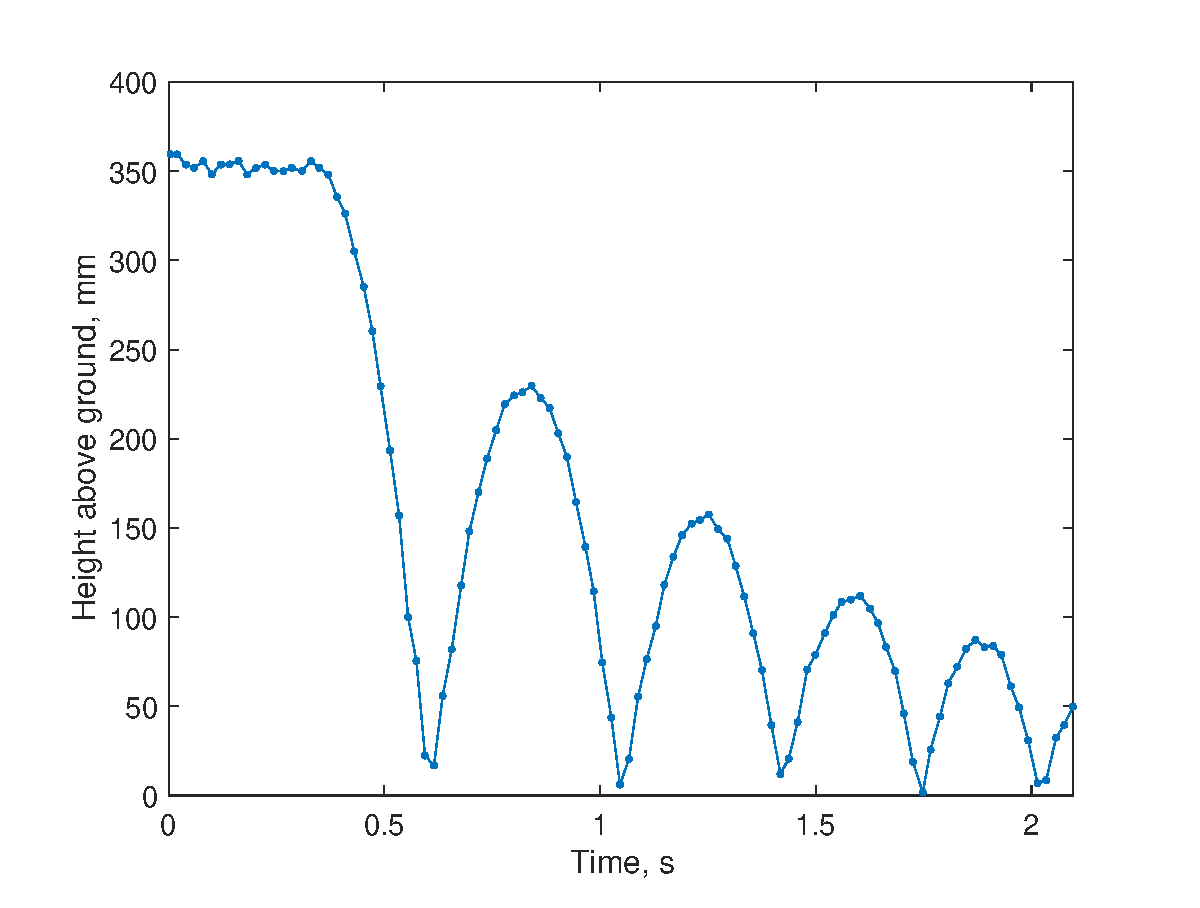
\includegraphics[width=\textwidth]{images/fig_bounce.eps}
        \caption{Plot of ball height over several bounces. The ball is dropped around $t = \SI{0.35}{\second}$.}
        \label{fig:bounce}
    \end{subfigure}\hfill
    \begin{subfigure}[t]{0.48\textwidth}
        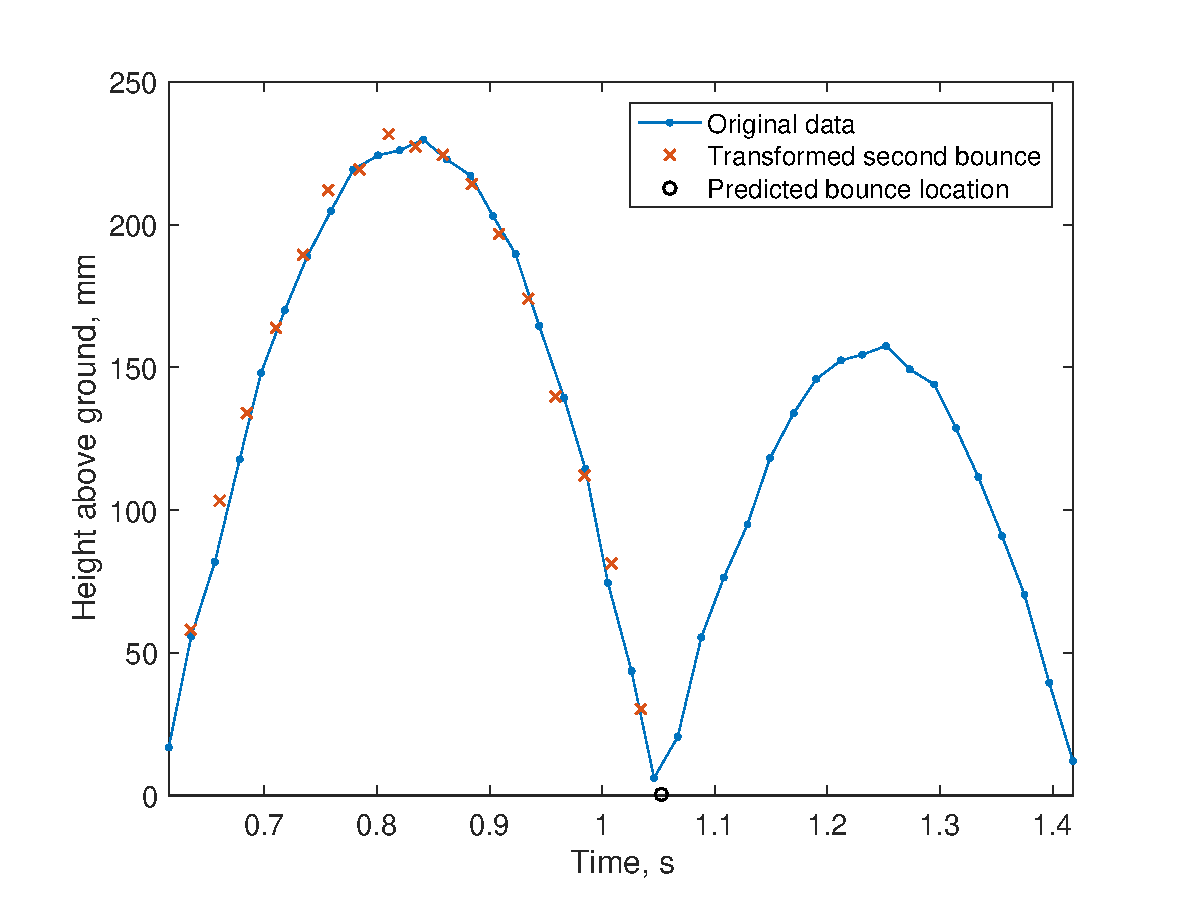
\includegraphics[width=\textwidth]{images/fig_transform.eps}
        \caption{Demonstration of the reflection and rescaling transform, using $R = 0.68$.}
        \label{fig:transform}
    \end{subfigure}
    \caption{\textbf{Kinematics of ball-bouncing.}}
\end{figure}

However, this introduced a new free parameter, $R$, that happens to be critical for accurate transformation. We could not estimate $R$ using linear regression, because the model was no longer linear: $z \sim \paren{\beta_0 + \beta_1 t + \beta_2 t^2} / R$. Thus, we were forced to either hard-code a value for the coefficient of restitution, attempt to minimize the mean-squared error among a range of $R$ values (since reasonable values of $R$ were between $0.2$ and $0.8$), or iteratively regress for better values of $R$ and $\v{\beta}$ using some form of block coordinate minimization. We initially attempted to implement the latter two algorithms, but in the late hours of Wednesday night / Thursday morning, something was wrong in our implementations, so we decided to hard-code a value of $R$ based on the surface and type of ball we were working with.

Finally, once the kinematic parameters were estimated, it was trivial to predict the location of the ball in global coordinates for any point in time in the future. Specifically, the landing location could be estimated by computing the roots of the $z$ polynomial, and by simple extension, the location of the ball at any height (since our paddle was vertically fixed) could be estimated using some more quadratic formulas.

\subsection{Omni-drive}
Let $\theta$ be the angle between global forward (the y-axis in \figref{fig:omni1}) and the current orientation of the robot (the direction specified by the line labeled ``F'' on the robot in \figref{fig:omni1}). Let $\alpha$ be the angle between global forward and the desired heading (the green line in \figref{fig:omni1}).
\begin{figure}[ht]
    \centering
    \includegraphics[width=0.6\textwidth]{images/omni1.pdf}
    \caption{\textbf{Global directions for omni-drive theory.}}
    \label{fig:omni1}
\end{figure}
Let $M1$, $M2$, etc. be the magnitude and direction of motors 1, 2, etc., where positive values indicate forward direction (the direction required to make the robot move forward relative to the robot’s orientation), and negative indicate backwards. The range of these values then is $[-1, 1]$.

The simple drive case is the one in which the robot is not rotating. In this case, $M1=M3$ and $M2=M4$. If we switch to a coordinate system aligned to the axis of the motors as in \figref{fig:omni2}, then it is clear that $\tan{\beta} = \frac{M2}{M1}$, where $\beta$ is the desired heading of the car relative to the new coordinate system. In terms of $\theta$ and $\alpha$, then, $\beta = \alpha - \theta + \frac{\pi}{4}$, so \[\tan{(\alpha - \theta + \frac{\pi}{4})} = \frac{M2}{M1}.\]

\begin{figure}[ht]
    \centering
    \includegraphics[width=0.6\textwidth]{images/omni2.pdf}
    \caption{\textbf{Relative directions for omni-drive theory.}}
    \label{fig:omni2}
\end{figure}

Allowing rotations of the car only complicates this slightly. Rotations can be achieved by simply offsetting the speeds of $M1$ and $M3$ relative to each other, and the same for $M2$ and $M4$. Let s be the speed of rotation from $[-1, 1]$. Then \[s = \frac{M2-M4}{2} = \frac{M3-M1}{2}.\]

When the car is rotating, the average of $M2$ and $M4$ remains constant for any $s$ and likewise for $M1$ and $M3$, so our original equation can now be rewritten as \[\tan\paren{\alpha - \theta + \frac{\pi}{4}} = \frac{(M2+M4)/2}{(M1+M3)/2} = \frac{M2+M4}{M1+M3}.\]

The final equation of motion is simply a constant that $\max\brace{M1, M2, M3, M4} = M$, where $M$ is the magnitude of movement in the direction specified by $\beta$. Together, these three equations, functions of $\alpha$, $\theta$, $s$, and $M$, fully specify the control of the four wheels.

\subsection{Accelerometer}
An accelerometer measures acceleration relative to its own orientation. Therefore, as the robot spins and the accelerometer spins with it, the accelerometer will not be measuring acceleration in a consistent direction. To get meaningful readings from the accelerometer, we need to use information about our orientation from the gyroscope to correctly project the accelerometer’s acceleration readings to global, constant axes. Further, the accelerometer is not mounted at the center of the robot, so as the robot spins, centrifugal force will add a false acceleration to the accelerometer. This acceleration needs to be subtracted off to get accurate readings.

Let $x\sub{raw}$ and $y\sub{raw}$ be the original readings of the accelerometer. First, we need to subtract off the effect of centrifugal force. As in \figref{fig:accel1}, let the angle between the negative $y$-axis and the accelerometer be $\alpha$, the distance between the center of mass of the robot and the accelerometer be $r$, and the rate of rotation be $\omega$. Then \[x_1 = x\sub{raw} + r{\omega^2}\cos{\alpha}\] and \[y_1 = y\sub{raw} + r{\omega^2}\sin{\alpha},\] where $x_1$ and $y_1$ are the adjusted accelerations.

\begin{figure}[ht]
    \centering
    \begin{subfigure}[t]{0.48\textwidth}
        \centering
        \includegraphics[height=0.4\textheight]{images/accel1.pdf}
        \caption{Definitions for centrifugal force corrections to accelerometer readings.}
        \label{fig:accel1}
    \end{subfigure}\hfill
    \begin{subfigure}[t]{0.48\textwidth}
        \centering
        \includegraphics[height=0.4\textheight]{images/accel2.pdf}
        \caption{Angle definitions for accelerometer theory.}
        \label{fig:accel2}
    \end{subfigure}
    \caption{\textbf{Definitions for accelerometer theory.}}
\end{figure}

Let $\theta$ be the angle between the accelerometer and global coordinates as in \figref{fig:accel2}. Then $y = x_1\cos{\theta} - y_1\sin{\theta}$ and $x = -x_1\sin{\theta} - y_1\cos{\theta}$, where $x$ and $y$ are global $x$ and $y$ accelerations. 

With these calculations, the global $x$ and $y$ accelerations can be double integrated to determine the position of the car at any time.

\clearpage
\section{Hardware}
\figref{fig:pics} shows photographs of the final product from various angles, annotated with important components.
\begin{figure}[H]
    \centering
    \begin{subfigure}[t]{0.8\textwidth}
        \includegraphics[width=\textwidth]{images/top.JPG}
        \caption{Top view.}
    \end{subfigure}

    \begin{subfigure}[t]{0.8\textwidth}
        \includegraphics[width=\textwidth]{images/bottom.JPG}
        \caption{Bottom view.}
    \end{subfigure}
\end{figure}

\begin{figure}[H]\ContinuedFloat
    \centering
    \begin{subfigure}[t]{0.8\textwidth}
        \includegraphics[width=\textwidth]{images/front.JPG}
        \caption{Front view.}
    \end{subfigure}

    \begin{subfigure}[t]{0.8\textwidth}
        \includegraphics[width=\textwidth]{images/left.JPG}
        \caption{Side view.}
    \end{subfigure}
    \caption{\textbf{Photographs of the final robot.}}
    \label{fig:pics}
\end{figure}

\figref{fig:blockdiagram} shows a block diagram of the hardware set-up.
\begin{figure}[ht]
    \centering
    \includegraphics[width=0.85\textwidth]{images/BlockDiagram.pdf}
    %TODO: block diagram
    \caption{\textbf{Block diagram of the hardware setup for ping pong.} Black connections indicate ground connections; red connections indicate power (both regulated and unregulated); all other connections indicate data connections (e.g. from the PSoC to the H-bridges and servo, various \iic connections). Green components indicate power-related components; red components indicate actuators; blue components indicate sensors.}
    \label{fig:blockdiagram}
\end{figure}

\subsection{Chassis}
The chassis consists of two decks of components: a lower deck for the motors, H-bridges, and power (voltage regulator) board; and an upper deck for the Raspberry Pi, PSoC, accelerometer/gyro, and mounting points for the mast, which contains the two Pixy cameras. Since we inherited Gordon and Pfleger's chassis from 2016, we re-used their lower deck after aesthetically modifying the H-bridges, replacing bent set screws from the wheel hubs, and replacing the power board with our own voltage regulator board. On the other hand, we completely re-designed the top deck to suit our purposes. See \figref{fig:topdeck} for the laser cutting template for the top deck:
\begin{figure}[ht]
    \centering
    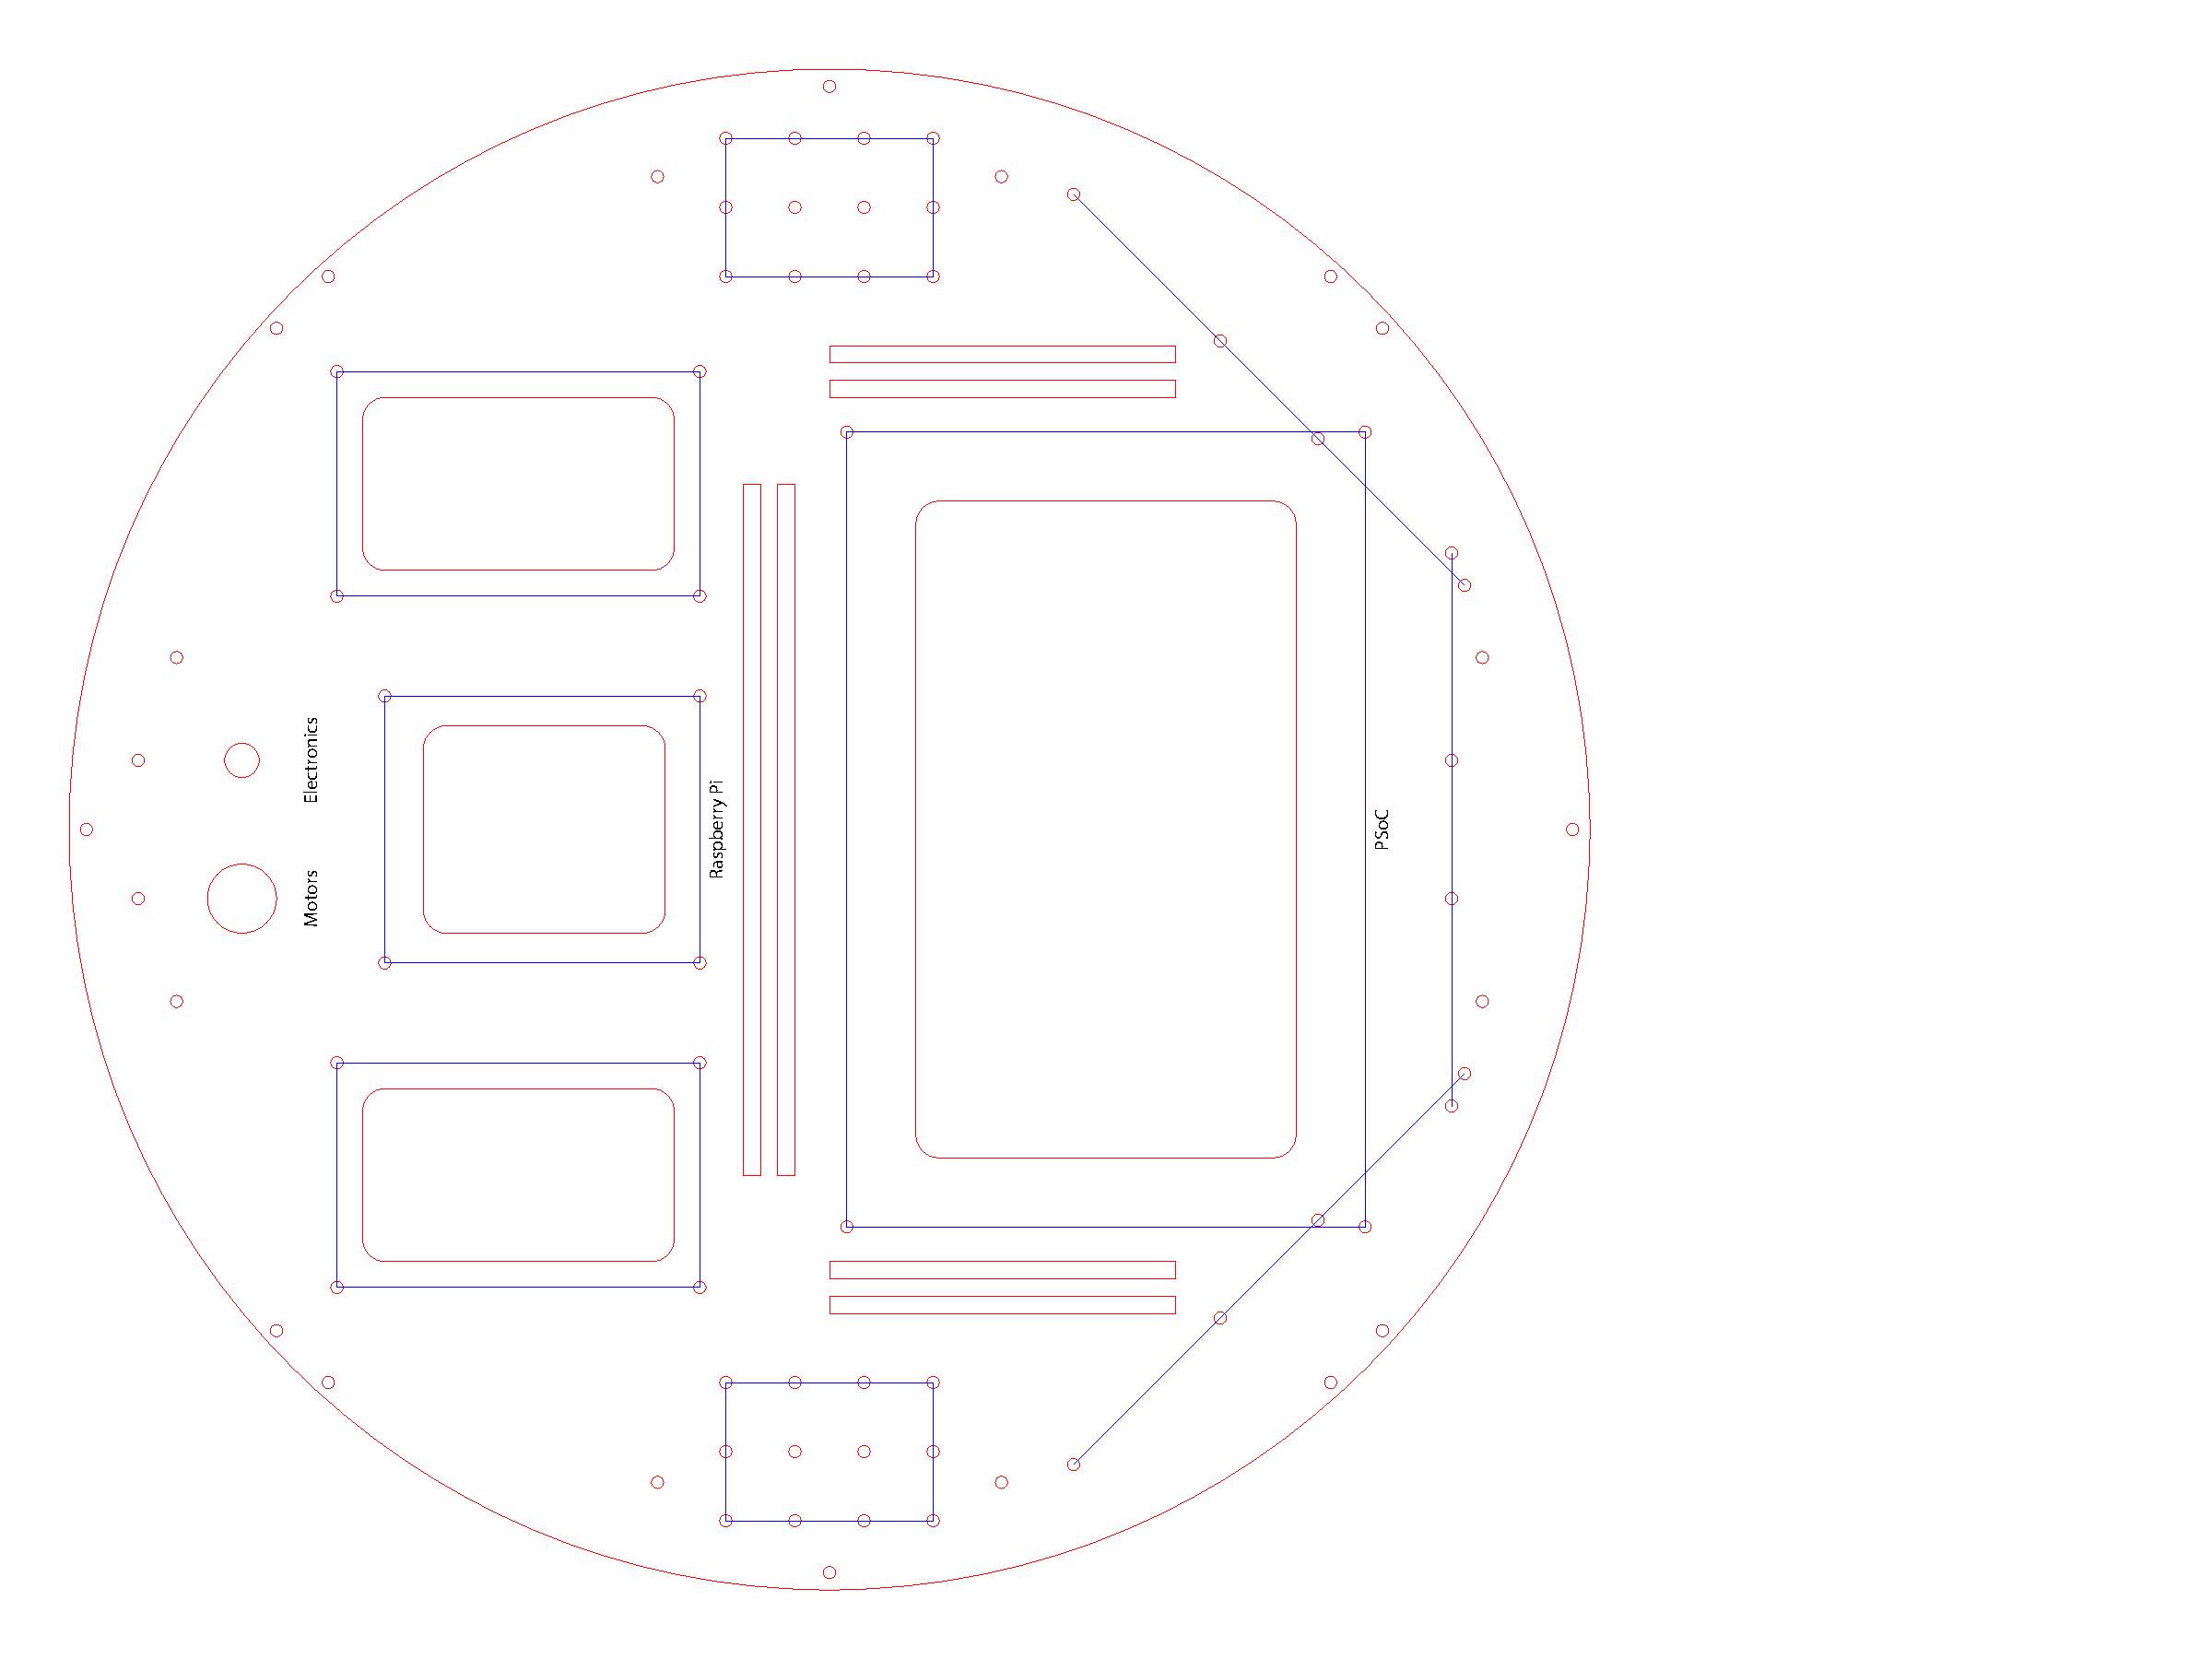
\includegraphics[width=0.7\textwidth]{images/topdeck.png}
    \caption{\textbf{Laser cut template for top deck.}}
    \label{fig:topdeck}
\end{figure}

We adapted the voltage regulator board from the speed control and navigation assignments: it has two linear \SI{5}{V} voltage regulators (LM7805) and many mounting points for both unregulated and regulated voltages (see \secref{sec:power} for details).

\subsection{Omni-wheel drive}
Because the ping-pong ball can land anywhere in space, we needed a robot that could quickly move anywhere in space. Because it is very difficult to do this with conventional steering systems, we decided to use an omni-directional drive (or omni-drive). An omni-drive consists of four wheels mounted at right angles to each other. These wheels have rollers along their circumference, allowing them to be pushed orthogonally to their direction of rotation. The rollers allow the robot to move in any direction, and the fact that the wheels can be independently controlled allows the sum of the forces to point in any direction. Together, this translates to a robot that can drive in any direction.

\subsubsection{Motors and chassis}
As mentioned previously in this report, we used an omni-drive chassis that had already been built last year by Ethan Gordon and Luke Pfleger. The main body is laser cut acrylic, with four 3D printed and acrylic motor mounts along the sides. The motors are \SI{22}{mm} diameter, $20.4:1$ geared, high power Pololu Gearmotors, and the wheels are 4'' VEX omni-wheels. All four motors are run off a single \SI{7.2}{\volt} NiCd battery. We made no real changes to this chassis, besides redoing some of the wiring and replacing the set screws for the wheels, as mentioned in the previous section.

\subsubsection{Motor controllers}
\label{sec:hbridge}
An omni-drive requires 4 independent controllers capable of driving forwards and backwards and controlling throttle. To do this, we use H-bridges. H-bridges use four transistors to completely select power and ground for each terminal of the motor as shown in \figref{fig:hb-dummy}. By turning on different transistors, the H-bridge can direct current through the motor in either direction, and can brake the motor by connecting both terminals to either power or ground. Since the switching is controlled by transistors, they can be given PWM signals, which allows for throttle control.

\begin{figure}[ht]
    \centering
    \begin{subfigure}[t]{0.48\textwidth}
        \centering
        \includegraphics[height=0.4\textheight]{images/hbridge.pdf}
        \caption{H-bridge dummy circuit diagram.}
        \label{fig:hb-dummy}
    \end{subfigure}\hfill
    \begin{subfigure}[t]{0.48\textwidth}
        \includegraphics[height=0.4\textheight]{images/hbridge-circuit.pdf}
        \caption{Actual H-bridge circuit diagram.}
        %TODO: this image
        \label{fig:hb-circuit}
    \end{subfigure}
    \caption{\textbf{H-bridge circuit diagrams.}}
    \label{fig:hbridge}
\end{figure}

This basic idea is very simple, but there are many complications in the design of an H-bridge. The first of these arises from our use of PWM signals. A PWM signal has both an ``on'' period and an ``off'' period. During the ``on'' period, one side of the motor must be connected to ground and the other must be connected to power. To make things concrete, let's assume we are driving the motor in a direction such that the left side is connected to ground and the right is connected to power. The question, then, is what to do during the ``off'' period. Since the motor has inductance, it is a bad idea to completely disconnect the motor during the ``off'' period, as this will force the back EMF to drop across the internal diodes of the transistors. Our remaining options then, are to reverse the motor during the ``off'' period, or to brake it. Reversing the motor during the ``off'' period is known as lock anti-phase drive, and braking it is known as phase-magnitude drive.

The second complication with H-bridges is that if two transistors on the same side of the H-bridge are ever turned on at the same time, they create a direct short from power to ground. The H-bridge, then, must be designed in such a way that two same-side transistors cannot be on at the same time.

The chassis we used also had H-bridges that had already been built. The circuit diagram and board image is shown in \figref{fig:hb-circuit}. NMOS transistors are used on the ground side, and PMOS transistors are used on the power side. Each gate has an inline \SI{1.1}{\kilo\ohm} resistor to protect the PSoC from back EMF spikes. The left side gates are wired directly together, as are the right side gates. Given a low signal, then, the PMOS will turn on and the NMOS will turn off, connecting the motor terminal to power. Given a high signal, the PMOS will turn off and the NMOS will turn on, connecting the motor terminal to ground. Since we never want to motor to be floating (as that causes the back EMF to drop across the FET diodes), this arrangement works well.

Since we are operating the motors at \SI{7.2}{\volts}, the PMOS transistors need an input close to that to turn off. The PSoC drives its outputs at \SI{3.3}{\volts} which is not nearly high enough to achieve this. The original design used open drain comparators with a threshold set at \SI{1.5}{\volts} to achieve the higher voltage. The \SI{750}{\ohm} pull-up resistors in the circuit diagram act as the pull-ups for the open-drain outputs. Since the PSoC has its own internally configurable open drain outputs, we simply used those to directly drive the H-bridges, eliminating the original comparators. The pull-up resistors also serve to connect both terminals of the motor to ground in the event of a PSoC failure, creating a safe failure condition.

Gordon and Pfleger used lock anti-phase drive, and this influenced several of their H-bridge design decisions. Since the ``off'' time PWM signal is in reverse, the stop condition for the motors is a $50\%$, duty cycle, such that the motor is connected forwards half the time and backwards the other half of the time. According to their report, the first time they tried this, with a fairly standard \SI{100}{\hertz} PWM, they burned out two motors. To avoid burning out their motors, they had to increase their frequency to about \SI{10}{\kilo\hertz} This high frequency required making the pull-up resistors very small, to make the time constant of the transistors' gate capacitances low enough to allow them to actually turn on and off with the input signal. We believe that the main cause of their motors burning out was their choice of phase anti-lock drive. The frequency was high enough that the motors did not turn, as intended, but was also low enough that there was enough time for the current to reach full stall current in each direction, thereby burning out the motors.

We chose to use phase-magnitude drive, if only for the simple reason that it is more efficient to brake the motor during the ``off'' time than it is to reverse it. This also came with the benefit that we believe we could have safely run the motors at a much lower PWM frequency, as the stop condition for phase-magnitude drive is simply braking without any PWM signal, so nothing can stall. We only apply a PWM signal when the motor is actually supposed to turn, so any frequency should be safe. If the motor were to actually stall, it is possible that the high frequency would help protect the motor, but otherwise, we believe a lower frequency would have been safe. However, we decided to leave the frequency at \SI{10}{\kilo\hertz}, since we knew that was absolutely safe. We did occasionally see some problems where the motor would have trouble starting at low speeds (for example, going from off to a $30\%$ duty cycle, the motor would occasionally stall briefly and require a push to get going). A lower frequency might have given the motor more sustained current and allowed it to start more reliably at lower speeds.

The specific details of the control signals \texttt{C1} and \texttt{C2} required to drive the H-bridge in sign-magnitude mode will be given when we discuss the hardware programmable hardware required to implement them in \secref{sec:prog-hard-motor}.

\subsection{Dead reckoning}
Since the very principle of an omni-drive's motion is dependent on the wheels slipping, we cannot track the wheels' motion to determine the position of our robot. Instead, we use dead reckoning. To implement dead reckoning, we use a 9-DOF combined accelerometer, gyroscope, and magnetometer, the LSM9DS0 chip from ST Microelectronics, mounted on an Adafruit breakout board. This chip communicates with the PSoC through \iic.

\subsection{Cameras and mast}
The CMUcam5 (Pixy camera, or simply ``Pixy'') is a low-cost computer vision system developed by CMU and Charmed Labs that can be easily trained to recognize colored objects. The Pixy uses the OV9715 CMOS WXGA (1-MP) image sensor, which supports $1280\times 800$ resolution at \SI{25}{fps} or $640\times 400$ resolution at \SI{50}{fps}. Because of the memory limitations of the on-board microcontroller and to achieve the higher frame rate, the CMUcam5 default firmware restricts the resolution to $640\times 400$. Furthermore, the object detection algorithm outputs object coordinates and dimensions at $320\times 200$ resolution.

The Pixy outputs its data either through USB (which can interface with the Raspberry Pi with the \texttt{libpixyusb} library provided), or various serial protocols such as SPI, \iic, and UART (it can even output as raw analog/digital). Initially, we attempted to interface with the Pixy cameras using SPI due to its speed, but because of bus collisions with two cameras (even with the chip-enable functionality), we decided to use \iic with two addresses.

The Pixy cameras were mounted \SI{8.5}{inches} apart on the mast at the front of the robot to permit stereo vision, and were connected to the Raspberry Pi with ribbon cables. See \figref{fig:mast} for the laser cut template of the camera mast. We included four possible mounting positions for the Pixy cameras: the top two were the intended mounting positions, but if the cameras were too high to detect the ball, we would have moved the cameras to the bottom two mounting positions. With the cameras on the top mounting positions, the cameras were approximately \SI{260}{mm} above the ground.

\begin{figure}[ht]
    \centering
    \includegraphics[width=0.8\textwidth]{images/mast.png}
    \caption{\textbf{Laser cut template for camera mast.}}
    \label{fig:mast}
\end{figure}

\subsection{Paddle mount}
We wanted to be able to control the angle of the ping-pong paddle as we hit the ball, so we needed to design a mount for the paddle that would allow a servo to rotate it. We used a Hitec HS-322HD servo, a very common hobby servo. We did not want the servo to be subjected to shear forces from the paddle, so our mount needed to constrain the paddle’s position, and only allow it to rotate. We decided the best way to do this would be to encase the servo's handle in a cylinder, and then let that cylinder rotate within another cylinder. The first cylinder evens out the surface of the handle, and then the second constrains its motion to just rotation.

The inner mount was made in two halves so that we could simply screw each half into the handle. See \figref{fig:paddle} for images of all the parts. The servo mounts right in line with the paddle, and directly drives its rotation. Once the servo is attached to the mount, the paddle simply slides into the mount and connects to the servo. We included two holes through the mount to allow a faceplate to be attached after the paddle is slid in, to stop the paddle from sliding out when the robot rotates. However, we did not have long enough screws or threaded rods to attach such a faceplate, so we instead ran some zip-ties across the face to secure the paddle.

\begin{figure}[ht]
    \centering
    \includegraphics[width=0.7\textwidth]{images/paddle.png}
    %TODO: this image
    \caption{\textbf{Images of 3D-printed paddle mount parts.}}
    \label{fig:paddle}
\end{figure}

The mount had to fit in a very tight area, so to avoid having to go through many iterations as we discovered clearance issues, we made a mock model of our robot that included everything we thought could be a clearance issue. The mock robot model is shown in wireframe in \figref{fig:mock}, with the inner mount in green, the outer mount in blue, and the servo in red. This assembly allowed us to successfully design the mount on our first try.

\begin{figure}[ht]
    \centering
    \includegraphics[width=0.7\textwidth]{images/mock.png}
    %TODO: this image
    \caption{\textbf{Wireframe mock model of robot for paddle mount assembly.}}
    \label{fig:mock}
\end{figure}

\subsection{Power supply}
\label{sec:power}
To power the electronics of the robot (all but the four omni-drive motors), we used a single \SI{9.6}{V} NiMH battery. Two linear voltage regulators provided power for the accelerometer board and the paddle servo motor (one regulator each), and unregulated \SI{9.6}{V} was provided to the PSoC (which had an internal regulator), the two Pixy cameras (which had their own regulators), and the Raspberry Pi via an adjustable output buck (DC-DC step-down) converter.

We initially attempted powered the Raspberry Pi with regulated \SI{5}{V} through the GPIO pins, because the \SI{5}{V} pins and ground are shared across the whole device. This is highly discouraged these rails are not protected, while the micro USB port is protected with a polyfuse (a resettable fuse). We quickly decided to adapt a spare micro USB cable so that the Raspberry Pi could be powered through the USB port. We also quickly discovered that the Raspberry Pi drew too much current (about \SI{0.1}{A} when idle, and up to about \SI{0.6}{A} when booting or compiling C++) to power from a linear voltage regulator: with a voltage drop of \SI{4.6}{V} and a current of \SI{0.5}{A}, a linear voltage regulator would dissipate about \SI{2.3}{W} of power when booting; the voltage regulator would heat up unacceptably even with a heatsink, and it depleted the batteries too quickly for acceptable usage. Because of this, we powered the Raspberry Pi through a Drok LM2595 analog control voltage controller (a DC-DC step-down converter). Conveniently, this converter also doubled as a battery level meter for the \SI{9.6}{V} battery.

\subsection{Programmable hardware}
\figref{fig:topdesign} shows the top-design of our programmable hardware in PSoC Creator 2.1.
\begin{figure}[ht]
    \centering
    \includegraphics[width=0.99\textwidth]{images/topdesign.pdf}
    \caption{\textbf{Top-design of the ping pong project.}}
    \label{fig:topdesign}
\end{figure}

\subsubsection{Hardware for motor control}
\label{sec:prog-hard-motor}
Phase-magnitude drive requires a PWM signal where the ``on'' time signal drives the motor in the intended direction and the ``off'' time signal brakes the motor. Since the H-bridge circuit as described in \secref{sec:hbridge} defaults to connecting each motor terminal to ground, this can be achieved by simply sending a normal PWM signal to one of the inputs \texttt{C1} or \texttt{C2} and letting the other input remain pulled high by the H-bridge circuit. When the PSoC drives \texttt{C1} low, the left terminal is connected to power and the motor goes forward, and when the PSoC releases \texttt{C1}, the left terminal is pulled back high an the motor brakes. To go in reverse, the PSoC simply needs to drive \texttt{C2} instead of \texttt{C1}.

This, then, breaks the control into two very natural signals, direction and magnitude. The PWM signal controls the magnitude of rotation, and changing which terminal it goes into controls the direction of rotation. We implemented this scheme in the programmable hardware with PWM blocks and demultiplexers (i.e., switches). There is one PWM block per motor, and each PWM block outputs into a demultiplexer which selects between forward and reverse based on a software control signal. The software control signals come from the \verb|Control_Reg_Direction| block. This is the complete picture of the control at a high level, but a couple more additions were required to make it actually work. The final control signal outputs of the PSoC are open drain, so ``on'' corresponds to a low signal and ``off'' corresponds to a high signal. Demuxes output low on all unused inputs, which is the opposite behavior to what is desired, so we had to invert all of the demux outputs to make them default to floating rather than pulling low. This also had the convenient effect of making the high side of the PWM signal correspond to driving the output low, which is what turns the motor on, so on the software side, the duty cycle maps directly to throttle rather than inversely.


\subsubsection{Other hardware}
The servo that controls the angle of the paddle is directly controlled by a single PWM block, \verb|PWM_Servo|. We continued to use a UART block to communicate with our computers for debugging, and added a second, \verb|Serial_Pi| to communicate with the Raspberry Pi. We also have a master I2C block that manages communication with the accelerometer/gyro chip. There is also a counter block, \verb|Counter_Refresh|, which is used as a refresh timer. It interrupts at a rate of \SI{1}{\kilo\hertz}. Finally, we have another counter, \verb|Counter_Time|, on a slower clock, that is used to accurately keep track of time.

\section{Software for PSoC}

\subsection{Omni-drive control}
%TODO: TJ

\subsection{Dead reckoning}
%TODO: TJ

\subsection{Paddle mount servo control}
%TODO: TJ

\section{Software for Raspberry Pi}
\subsection{Pixy camera communication}
Initially, to implement SPI communication with a single Pixy camera, we adapted the code from this GitHub repository: \url{https://github.com/omwah/pixy_rpi}. This has an implementation of SPI communication using \verb|wiringPiSPI.h| from the \verb|WiringPi| library by Gordon Henderson, as well as a general Pixy data processing interface using the object block format found in the Porting Guide of the Pixy camera: \url{http://cmucam.org/projects/cmucam5/wiki/Porting_Guide}. The files are organized such that \verb|Pixy.h| defines the class \verb|LinkSPI|, which abstracts the communciation protocol with the SPI interface, \verb|TPixy.h| defines the class \verb|TPixy|, which abstracts the object block protocol further and maintains a buffer of received blocks, and \verb|echo.cpp| uses the \texttt{TPixy} class defined in \texttt{TPixy.h} to echo blocks to standard output. Abstracted in this way, the client code becomes very simple:
\begin{minted}[breaklines]{c}
#include <Pixy.h>

Pixy pixy;

int main() {
    int j;
    uint16_t blocks;
    while (true) {
        blocks = pixy.getBlocks();
        if (blocks) {
            std::cout << "Detected " << blocks << std::endl;
            for (j = 0; j < blocks; j++) {
                std::cout << "  block " << j << " ";
                pixy.blocks[j].print();
            }
        } else {
            std::cout << "No blocks detected" << std::endl;
        }
    }
    return 0;
}
\end{minted}

As mentioned earlier, however, SPI proved not flexible enough for communication with two Pixy cameras---at least in the \texttt{WiringPi} implementation of the SPI library---so we transitioned to \iic. This transition ended up being rather simple, because we only had to change a handful of functions to handle the difference in endianness, and to use the \verb|WiringPiI2C.h| header instead. The full implementation communication code can be found in the appendix.

\subsection{Stereo vision}
%TODO: BC

\subsection{Trajectory estimation}
%TODO: BC

\subsection{Serial communication}
%TODO: update (TJ)
We continued to use serial communication extensively to debug the camera and navigation portions of our program and to adjust our PID variables. We also moved to using the DB9 header only for bench testing and a wireless XBee serial communication chip for track testing. We changed nearly no code or programmable hardware to move to the XBee, since it relied on the same UART communication as the DB9.

We heavily updated our list of serial commands to improve memorability and consistency, and to expand to control camera and navigation parameters. Our updated commands are listed in \tblref{tbl:commands}.
\begin{table}[ht]
    \centering
    \begin{tabular}{@{}ll@{}}
        \toprule
        \textbf{Command} & \textbf{Description} \\ \midrule
        \texttt{CTx} & Change throttle \\
        \texttt{GS} & Get all variables associated with speed control \\
        \texttt{TS} & Toggle speed PID control \\
        \texttt{TDC} & Toggle distance timeout for speed control \\
        \texttt{TDS} & Toggle dynamic speed control \\
        \texttt{CPSx} & Change proportional term for speed control \\
        \texttt{CISx} & Change integral term for speed control \\
        \texttt{CDSx} & Change derivative term for speed control \\
        \texttt{CSSx} & Change steady-state throttle for speed control \\
        \texttt{CTSx} & Change target speed for speed control \\
        \texttt{CTDx} & Change target distance for speed control \\
        \texttt{TVS} & Toggle verbose printout for speed PID control \\ \midrule
        \texttt{GC} & Get all camera variables \\
        \texttt{RC} & Reset camera variables \\
        \texttt{CSx} & Change steering/servo direction \\
        \texttt{CMMx} & Change maximum permitted line misses \\ \midrule
        \texttt{TN} & Toggle navigation PID control \\
        \texttt{CPLx} & Change proportional term for line position error \\
        \texttt{CILx} & Change integral term for line position error \\
        \texttt{CIILx} & Change double integral term for line position error \\
        \texttt{CDLx} & Change derivative term for line position error \\
        \texttt{CPTx} & Change proportional term for angle error \\
        \texttt{CITx} & Change integral term for angle error \\
        \texttt{CDTx} & Change derivative term for angle error \\
        \texttt{CTSNx} & Change nominal target speed for navigation \\
        \texttt{TLE} & Toggle line error tracking \\
        \texttt{TVN} & Toggle verbose printout for navigation PID control \\ \midrule
        \texttt{A} & Abort (kill speed and navigation PID control) \\ \bottomrule
    \end{tabular}
    \caption{\textbf{Table of serial interface commands.}}
    \label{tbl:commands}
\end{table}

\section{Results}
See \tblref{tbl:pid} for the final PID coefficients we used. We updated our coefficients from speed control because we are no longer dynamically updating the target speed to reach the distance in a specific time. We used only the proportional and derivative terms for line position and angle (no integral terms), and unfortunately, despite our efforts to calculate it accurately, the angle contributed very little to our control. Given more time, we may have been able to develop a better system of control to more robustly control steering at higher speeds.
\begin{table}[ht]
    \centering
    \begin{tabular}{@{}rlll@{}}
        \toprule
        & \textbf{P} & \textbf{I} & \textbf{D} \\ \midrule
        Speed control & $80.0$ & $1.0$ & $10.0$ \\
        Line position & $3.0$ & $0.0$ & $2.0$ \\
        Line angle & $0.5$ & $0.0$ & $0.0$ \\ \bottomrule
    \end{tabular}
    \caption{\textbf{Final PID coefficients}}
    \label{tbl:pid}
\end{table}

See \tblref{tbl:times} for our final times for one lap. The highest speed we managed to achieve was with a nominal \SI{6.0}{ft/s}, though by reducing speed while turning corners, our average speed was only about \SI{5.4}{ft/s}. We were unfortunately unable to consistently replicate this speed, and we performed our demo with a nominal target speed of \SI{4.0}{ft/s}.
\begin{table}[ht]
    \centering
    \begin{tabular}{@{}lll@{}}
        \toprule
        \textbf{Nominal target speed} & \textbf{Time for one lap} & \textbf{Average lap speed} \\ \midrule
        \SI{4.0}{ft/s} & \SI{28}{s} & \SI{3.8}{ft/s} \\
        \SI{5.0}{ft/s} & \SI{22}{s} & \SI{4.9}{ft/s} \\
        \SI{6.0}{ft/s} & \SI{19.96}{s} & \SI{5.4}{ft/s} \\ \bottomrule
    \end{tabular}
    \caption{\textbf{Time trial results}}
    \label{tbl:times}
\end{table}

\section{Further work}
%TODO: BC: more robust ball tracking, more robust movement accuracy and location tracking, more robust UART communication, some sort of PID control with global coordinates and camera coordinates so that position could be updated in real time

\clearpage
\section{Appendix: full listings}
\etocsetnexttocdepth{2}
\etocsettocstyle{\subsection*{Contents}}{}
\cftsubsubsecindent 0pt
\localtableofcontents

\subsection{\texttt{main.c}}
% \begin{mdframed}[backgroundcolor=bg]
%     \inputminted[breaklines]{c}{files/main.c}
% \end{mdframed}


\end{document}
